\documentclass[10pt]{beamer}
\usetheme{Madrid}
\usepackage[utf8]{inputenc}
\usepackage{amsmath}
\usepackage{amsfonts}
\usepackage{amssymb}
\usepackage{graphicx}
\usepackage{hyperref}

\usepackage{pgfpages}
\usepackage{ragged2e}
\usepackage{tikz}
\usetikzlibrary{automata,arrows,positioning,calc}

\newif\ifplacelogo % create a new conditional
\placelogotrue % set it to true
\logo{\ifplacelogo
\includegraphics[width=0.2\textwidth]{imgs/optum_logo.jpg}\fi} % replace with your own command

\author[PM]{Pietro Mascolo}
\title[Predicting the future]{Predicting future states using Markov Chains}
%\setbeamercovered{transparent} 
%\setbeamertemplate{navigation symbols}{} 
%\logo{
\includegraphics[width=0.2\textwidth]{imgs/optum_logo.jpg}} 
\institute[Optum]{\textbf{\Large{Optum Ireland Ltd.}}} 
\date{\tiny{April 22, 2018}}

\definecolor{optum-orange}{RGB}{232, 119, 34}
\definecolor{optum-green}{RGB}{7,133,118}
\definecolor{optum-yellow}{RGB}{234,170,0}
\definecolor{optum-gray}{RGB}{136,139,141}
\definecolor{optum-link-blue}{RGB}{0,102,204}

\mode<presentation>
 {
 \setbeamercolor*{palette primary}{use=structure,fg=white,bg=optum-orange}
 \setbeamercolor*{palette secondary}{use=structure,fg=white,bg=optum-gray}
 \setbeamercolor*{palette tertiary}{use=structure,fg=white,bg=optum-yellow}
 \setbeamercolor*{block title}{use=structure,fg=white,bg=optum-green}
 }
 
%\setbeameroption{show notes on second screen=right}

\newtheorem{customDefinition}{Definition}

%\subject{} 
\begin{document}

	\begin{frame}
		\titlepage
	\end{frame}

%\begin{frame}
%\tableofcontents
%\end{frame}

	\section{Introduction}
	
	\begin{frame}{What I'm going to tell you}
	\placelogofalse

		\begin{itemize}
			\item Introduction;
			\item definition and representation of Markov Chains;
			\item how Markov Chains can be used;
			\item a bit of Maths;
			\item a bit of code...
		\end{itemize}
		
		\begin{center}
		\vspace{0.5cm}
		Slides and code:\\
		\href{http://bit.ly/2H8giAW}{\structure{http://bit.ly/2H8giAW}}
		\end{center}
	\end{frame}

	\begin{frame}{Who I am}
		\begin{columns}
			\column{0.5\textwidth}
			\begin{itemize}
   				\item Physicist;
   				\item Data Scientist;
   				\item \textbf{Python enthusiast};
   				\item \textbf{Kotlin}/Scala practitioner;
   				\item \textbf{Golang} padawan;
   				\item Ham Radio Operator (EI/IZ4VVE);
   				\item Hiker;
   				\item Karateka;
   				\item Amateur Photographer;
   				\item ...
			\end{itemize}
   			
   			\column{0.5\textwidth}
   			\begin{flushright}
   			
   			
   				
\includegraphics[width=0.83\textwidth]{imgs/me.png}
			\end{flushright}
		\end{columns}
	\end{frame}
	
	
	\begin{frame}{Optum - Our mission}
		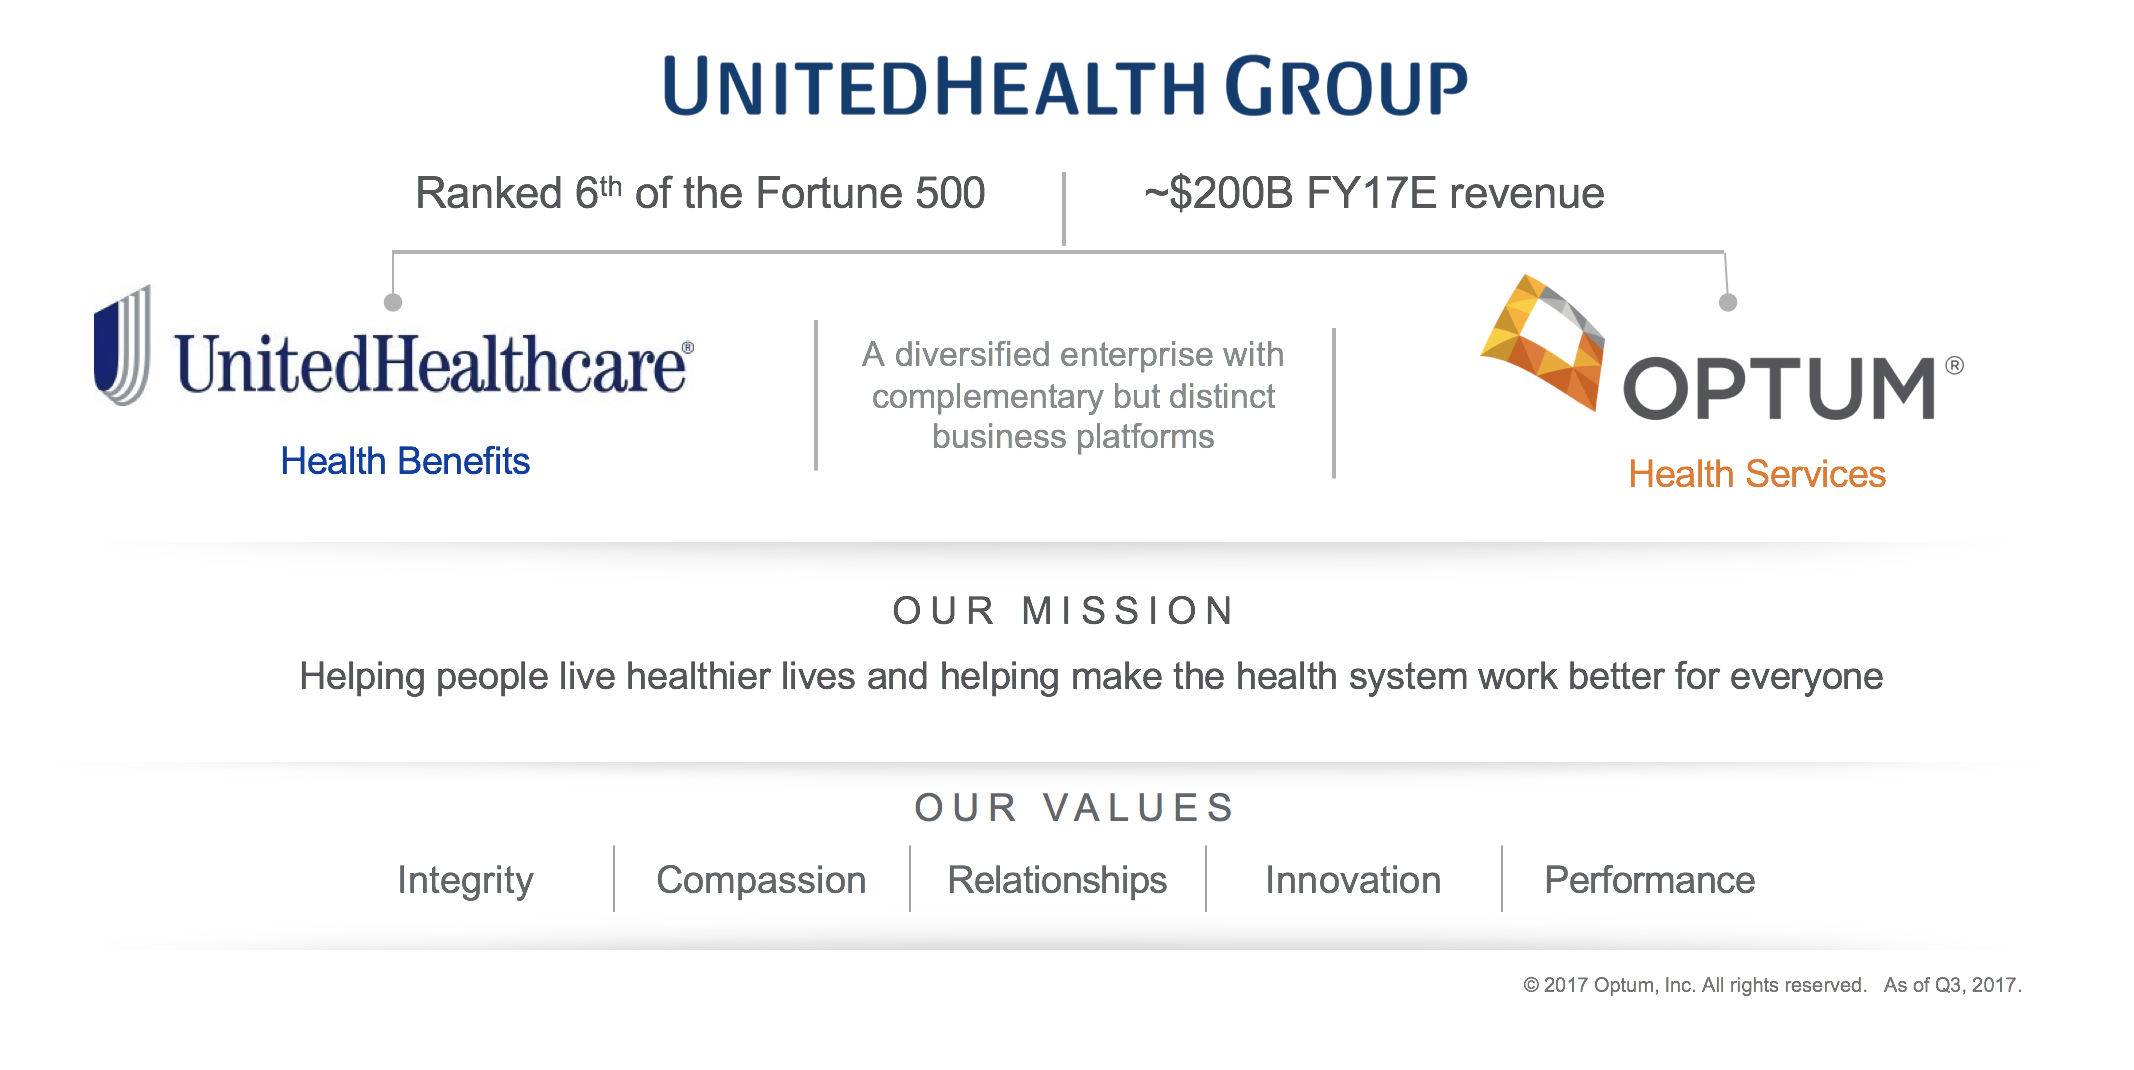
\includegraphics[width=\textwidth]{imgs/optum-mission.png}
		\note{6th in Fortune500, 270K employees as of 2018, 200B USD revenue}
	\end{frame}
	
	
	\section{Markov chains}
	
	\begin{frame}{Why all this?}
	 \begin{block}{Problem statement (sorry for having to "anonymise" everything...)}
		For each user of a system, a sequence of events occurs. Some sequences are good, some are bad. We want to determine driving factors of bad sequences as well as when/where they occur in the system, and for which users.
	 \end{block}
	\end{frame}		
	
	\subsection{Definition}

	\begin{frame}{Markov Chains - definition and representation 1/2}
		\only<1-3>{
			\begin{customDefinition}
				A [first order] Markov chain is "a stochastic model describing a sequence of possible events in which the probability of each event depends only on the state attained in the previous event."\footnotemark
			\end{customDefinition}
		}
		\uncover<2-3>{
			\begin{center}
				\Huge{\textbf{Don't panic!}}
			\end{center}
		}
		\only<3>{
			\begin{center}
				Everything will be clearer with an example...
			\end{center}
		}
		\uncover<4->{
			Let us imagine we have the following sequence: \\
			$$1, 2, 1, 2, 1, 2, 3, 1, 2$$
		}
		\uncover<5>{
			Based on these numbers we can say that:
			\begin{itemize}
				\item If the current state is $1$, there is a $100\%$ probability of moving to state $2$;
				\item if the current state is $2$, there is $66\%$ probability of evolving to state $1$ and $33\%$ of evolving to state $3$;
				\item if the current state is $3$, there is a $100\%$ probability of evolving to state $1$.
			\end{itemize}
		}
		
		\footnotetext[1]{From US English dictionary by Oxford Dictionaries.}
		
	\end{frame}
	
	\begin{frame}{Markov Chains - definition and representation 2/2}
		The states we have determined can be represented in a more visual fashion by using a matrix (or - even better - a graph).\\
		
		\begin{block}{Two representations}
		\begin{columns}[T]
			
			\column{0.48\textwidth}
			\vspace{0.1cm}
			\textbf{Matrix representation}
			\vspace{0.5cm}
			$$
			T = 
			\begin{pmatrix}
				0    & 1   & 0    \\
				0.66 & 0   & 0.33 \\
				1    & 0   & 0
			\end{pmatrix}
			$$
			%\end{block}%
			
			\column{0.48\textwidth}
			\vspace{0.1cm}
			\textbf{Graph representation}
			%\begin{block}{Graph representation}
				\begin{center}
					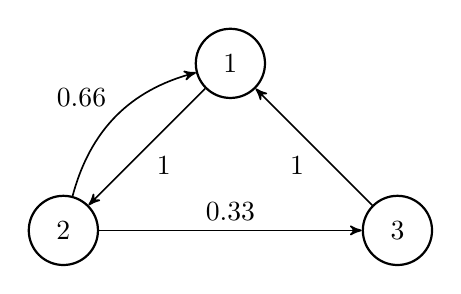
\begin{tikzpicture}[->, >=stealth', auto, semithick, node distance=3cm]
						\tikzstyle{every state}=[fill=white,draw=black,thick,text=black,scale=1]
							\node[state]    (1)                     {$1$};
							\node[state]    (2)[below left of=1]   {$2$};
							\node[state]    (3)[below right of=1]   {$3$};
							\path
								(1) edge   			node{$1$}         (2)
								(2) edge[bend left]  node{$0.66$}      (1)
									edge             node{$0.33$}      (3)	
								(3) edge             node{$1$}         (1);

					\end{tikzpicture}
				\end{center}
			
			\end{columns}
			\end{block}
	\end{frame}

	
	\subsection{Maths}
	
	\begin{frame}{A bit of Maths 1/3 - description}
		\only<1>{Now we need a bit of maths to show what we can do with Markov Chains...}
		\uncover<2->{
			We can describe a Markov Chain as follows: \\
			
			Given a set of possible states: $S=\{s_1, s_2, ..., s_n\}$, at each step, a generic state $i$ can move to a new state $j$ or remain in the same initial state with certain \textit{\structure{transition probabilities}}: \\
			\begin{center}
					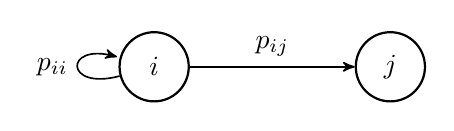
\begin{tikzpicture}[->, >=stealth', auto, semithick, node distance=3cm]
						\tikzstyle{every state}=[fill=white,draw=black,thick,text=black,scale=1]
							\node[state]    (i)                     {$i$};
							\node[state]    (j)[right of=i]   {$j$};
							\path
								(i) edge[loop left]  node{$p_{ii}$}      (i)
									edge             node{$p_{ij}$}      (j);
					\end{tikzpicture}
				\end{center}
		}
	\end{frame}
	
	\begin{frame}{A bit of Maths 2/3 - transition probabilities and next state}
		\only<1-2>{
			All the transition probabilities can be collected in a \structure{transition matrix}:\\
			$$
			T = \begin{pmatrix} 
   	 		p_{11} & \dots  & p_{1n}\\
    			\vdots & \ddots  &\\
    			p_{n1} &    &    p_{nn} 
    			\end{pmatrix}
    			$$
    			
    			\uncover<2>{
    				And given an initial state, the next state transition probabilities are given by:
    				$$
    				\mathbf{S_i^T} \times \mathbf{T} = \mathbf{S_j}
    				$$
    				
%    				and for $n$ time steps (for square transition matrices):
%    				$$
%    				\mathbf{S_i^T} \times \mathbf{T}^n = \mathbf{S_j}
%    				$$
    			}
		}

	\end{frame}
	
	\begin{frame}{A bit of Maths 3/3 - High order Markov Chains}
	
	\only<1>{So far we only treated first order Markov Chains: now we can expand on that!\\
	What will the next state be, given that the current state is $j$ \textbf{AND} the previous state was $i$?\\
	
	The transition matrix can be computed the same way as before, only considering all subsequent pairs in the sequence of states.\\}
	
	\uncover<2->{
		In case of a second order chain, the transition matrix will be of size $N(N-1) \times N(N-1)$, where $N$ is the cardinality of the set of possible states, and it will relate pairs of states instead of single states.\\
		
		$$
			T = \begin{pmatrix} 
   	 		p_{(11)(11)} & \dots  & p_{(11)(1n)}\\
    			\vdots & \ddots  & \\
    			p_{(n1)(11)} &    &    p_{(nn)(nn)} 
    			\end{pmatrix}
    		$$
	}
	\end{frame}
		
	\section{Code and live demo}
	
	\begin{frame}{Code and demo!! :D}
	
	\begin{center}
	\href{http://localhost:8888/notebooks/notebooks/Pycon9_MarkovChains.ipynb}{\structure{\Huge{Demo!}}}
	\end{center}
	\end{frame}
	
	
	\section{Conclusions}
	
	\begin{frame}{Q/A}
		\begin{center}
		
\includegraphics[width=0.9\textwidth]{imgs/qa.png}
		\end{center}
	\end{frame}	
	
	
	\begin{frame}{You've made it through!!}
		\begin{center}
		\Huge{Thanks for your attention!\\}
		\href{mailto:pietro_mascolo@optum.com}{\structure{\large{pietro\_mascolo@optum.com}}}
		\end{center}
	\end{frame}

\end{document}